\documentclass[12pt,a5]{bxjsarticle}

\usepackage{xltxtra}
\setmainfont{IPAPMincho}
\setsansfont{IPAPGothic}
\setmonofont{IPAGothic}
\XeTeXlinebreaklocale "ja"

\usepackage{hyperref}
\usepackage{listings}
\usepackage{verbatim}

\newcommand{\e}{\mathrm{e}}

\title{物理学情報処理論2 problem10}
\date{}

\begin{document}
\maketitle

\section{}

\[
  \frac{\partial u}{\partial t} = \sigma \frac{\partial^2 u}{\partial x^2}
\]
を解く。

対応する解
\[
  u(x, t) = \frac{1}{\sqrt{4\pi\sigma(t+t_0)}}\exp(-\frac{(x-5)^2}{4\sigma(t+t_0)}), t_0 = 1
\]
と共にグラフに描くと以下のようになる。

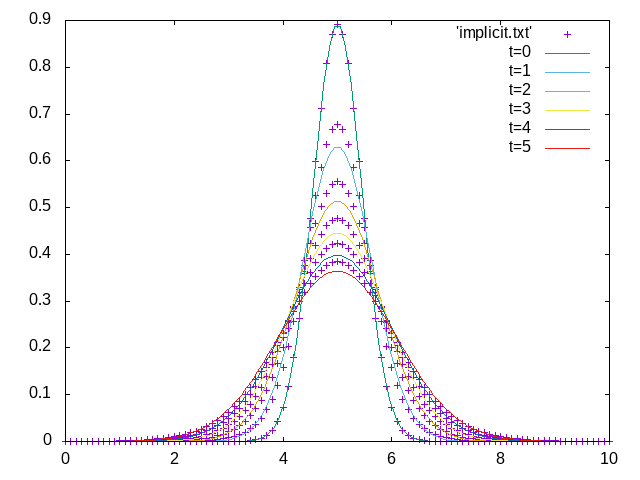
\includegraphics[width=\linewidth]{graph.png}

$ L = 5/3 $と$ L = 1/3 $の時、$ \theta $を動かして誤差を描くと以下のようなグラフとなる。

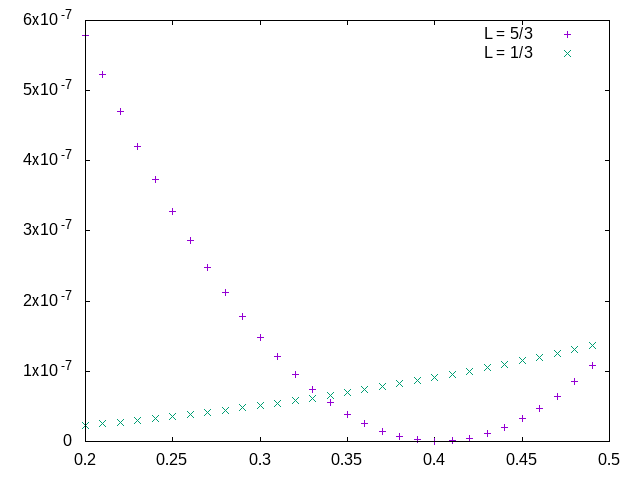
\includegraphics[width=\linewidth]{errors.png}

$ L = 5/3 $の時、$ \theta = 0.4 $付近で最小となることがわかる。

以下のスクリプトを用いて、orbit.datから図を生成した。
\lstinputlisting[caption=plot.sh,language=bash]{plot.sh}

\end{document}
